% *********************************************************************
% © 2016–2026 Jeremy Sylvestre
%
% Permission is granted to copy, distribute and/or modify this document
% under the terms of the GNU Free Documentation License, Version 1.3 or
% any later version published by the Free Software Foundation; with no
% Invariant Sections, no Front-Cover Texts, and no Back-Cover Texts. A
% copy of the license is included in the appendix entitled “GNU Free
% Documentation License” that appears in the output document of this
% PreTeXt source code. All trademarks™ are the registered® marks of
% their respective owners.
%
% *********************************************************************
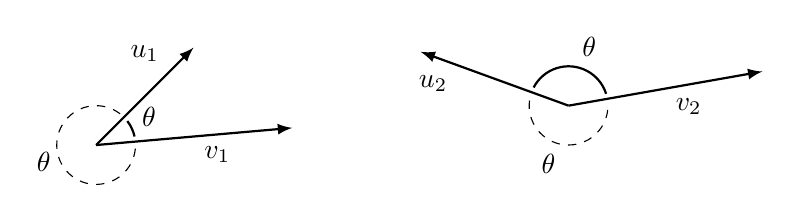
\begin{tikzpicture}[
	point/.style={circle,draw,very thin,fill,inner sep=0pt,minimum size=4pt},
	vector/.style={-latex},
]
	\draw[vector,thick] (0,0) to node[above left,near end] {$\uvec{u}_1$} ++(45:1.75cm);
	\draw[vector,thick] (0,0) to node[below right] {$\uvec{v}_1$} ++(5:2.5cm);
	\draw[thick] (0,0) ++(12.5:0.5cm) arc (12.5:37.5:0.5cm) node[right,midway,yshift=0.15cm] {$\theta$};
	\draw[dashed] (0,0) ++(52.5:0.5cm) arc (52.5:357.5:0.5cm) node[left,midway] {$\xcancel{\theta}$};
	\begin{scope}[xshift=6cm,yshift=0.5cm]
		\draw[vector,thick] (0,0) to node[below left,near end] {$\uvec{u}_2$} ++(160:2cm);
		\draw[vector,thick] (0,0) to node[below right] {$\uvec{v}_2$} ++(10:2.5cm);
		\draw[thick] (0,0) ++(17.5:0.5cm) arc (17.5:152.5:0.5cm) node[above right,midway] {$\theta$};
		\draw[dashed] (0,0) ++(172.5:0.5cm) arc (172.5:357.5:0.5cm) node[below left,midway] {$\xcancel{\theta}$};
	\end{scope}
\end{tikzpicture}
